
\chapter{The Riemann--Roch theorem}\label{RiemannRochChapter}

\section{How many sections?}

To study curves via their maps to projective spaces, we want to estimate the dimension of the space of global
sections of an invertible sheaf $\cL$. The beginning
of the story is the Riemann--Roch theorem.

Though we would like to be able to compute $h^0(\sL)$, it is much
easier to compute the 
Euler characteristic
\index{Euler characteristic}%
$$
\chi(\sL)\colonequals \sum_{i\geq 0} (-1)^i h^i(\sL).
$$
This computes $h^0(\cL)$ itself in many cases, by virtue of the following result:

\begin{theorem}[Serre--Grothendieck vanishing theorem]
\label{Serre--Grothendieck vanishing}
\index{Serre--Grothendieck vanishing theorem}%
\index{vanishing theorem!Serre--Grothendieck}%
If $\sF$ is a coherent sheaf on a projective scheme $X$ of dimension $n$, then for any $i$, the vector space $H^i(\sF)$ is finite-dimensional, and is 0 if  $i> n$. Moreover,
if $X\subset \PP^m$ then for $d\gg 0$, $\sF(d)$ is generated by its global sections and $H^i(\sF(d)) = 0$ for all $i>0$.\qed
\unif
\end{theorem}

\begin{proof}
This is a combination of 
theorems due to Grothendieck and Serre. See
\cite[Theorems III.2.7 and III.5.2]{Hartshorne1977}, 
and
also \cite{Serre1955} for a 
reasonably
concrete proof.
\end{proof}

A 
shortcoming
of this vanishing theorem is the lack of a bound on the number $d$ needed to achieve the second assertion. For smooth curves
and invertible sheaves
this is corrected by Theorem~\ref{RR theorem}, which gives a bound in terms of the genus and the degree.

One easy consequence of Theorem~\ref{Serre--Grothendieck vanishing} is
\vadjust{\allowbreak}%
that on a smooth variety the groups of invertible sheaves and divisor
\vadjust{\allowbreak}%
classes are the same (see also~\cite[Proposition
II.6.13]{Hartshorne1977}). 

\begin{corollary}\label{invertible sheaves and divisors}
If $X$ is a projective variety that is nonsingular in codimension $1$,
every invertible sheaf $\cL$ on $X$ is of the form $\cL =\cO_C(D)$ for some 
\index{Cartier divisor}\index{divisor!Cartier}%
Cartier divisor $D$ on $X$. Thus if $X$ is a smooth projective variety
\index{div|defi}%
the map $\div$ is an isomorphism from the group of invertible sheaves
to the group 
of divisor classes.
\unif
\end{corollary}

\begin{proof}
Let $H \subset \PP^r$ be a general hyperplane, and $E$  the divisor  of intersection of $C$ with $H$. We know that for $n \gg 0$, $\cL(n)$ has sections; and if $F$ is the divisor of zeroes of one such section, we have
$$
\cL = \cO_C(F - nE).
$$
If $X$ is smooth, then, since a regular local ring is a unique
factorization domain, every codimension 1 subvariety is defined locally 
by a single nonzerodivisor, and thus corresponds to a Cartier divisor.
This implies that $\div$ is surjective. Furthermore any 
isomorphism between invertible sheaves
\index{invertible sheaf!isomorphism between -s}%
is defined by multiplication with a global rational function, so that invertible sheaves defining linearly equivalent divisors are
isomorphic. Thus $\div$ is injective as well.
\end{proof}

\subsection*{Riemann--Roch without duality}

It follows from Theorem~\ref{Serre--Grothendieck vanishing} that on
any scheme $X\subset \PP^r$ we have $\chi(\sL(d)) = h^0(\sL(d))$ for
large $d$, 
and that $\chi(\sL) = h^0(\sL) - h^1(\sL)$ in the case of a curve.

\begin{theorem}[easy Riemann--Roch]\label{easy RR}
If $C$ is a smooth projective curve, and $\sL$ is an invertible sheaf on $C$, then $\chi(\sL) = \deg \sL + \chi(\sO_C)$.
\index{Riemann--Roch theorem!easy}%
\unif
\end{theorem}

\begin{proof}
 The result is tautological if $\sL = \sO_C$. Every invertible sheaf on $C$ has the form $\sL = \sO_C(D)$ for some
divisor $D$. If $p\in C$, then writing $\kappa(p)$ for the
structure sheaf of the subscheme $p\in C$, the long exact sequence in cohomology
associated to the short exact sequence
$$
0\to \sL(-p) \to \sL \to \sL\otimes \kappa(p)\to 0
$$
together with the isomorphism $\sL\otimes \kappa(p) \cong \kappa(p)$
and the vanishing of higher cohomology of a sheaf with zero-dimensional support allows us to compute 
$$
\chi(\sL) = \chi(\sL(-p)) + \chi(\kappa(p)) = \chi(\sL(-p)) + 1.
$$
Since every divisor on $C$ can be reached by adding and subtracting points, this suffices.
\end{proof}

Since the Euler characteristic of a sheaf is well-behaved, we can extend the result of Theorem~\ref{easy RR} 
to invertible sheaves on any one-dimensional scheme $C$, by defining
$\deg \sL \colonequals \chi(\sL) -\chi(\sO_C)$.
We will use this definition to express the self-intersection of a divisor on a surface in Section~\ref{surface basics}.

We can make the Riemann--Roch theorem still more useful by understanding the error term $h^1(\sL)$. This requires
the canonical divisor and Serre duality, to which
we now turn.


\section{The most interesting linear series}\label{most interesting}

The most important vector bundles on a manifold are the tangent and cotangent bundles. For reasons that
\index{cotangent bundle}%
will become clear, the focus in algebraic geometry is on the cotangent
bundle or, equivalently, the sheaf of differential 1-forms. On a
smooth curve $C$ the \emph{canonical sheaf} is the sheaf of
differentials, which is an 
\index{canonical sheaf}\index{sheaf!canonical}\index{sheaf!of differentials}%
invertible sheaf; on a smooth
variety of dimension $n$ we define the canonical sheaf to be the 
$n$-th exterior power of the sheaf of differentials. A section of 
$\omega_C$ is thus a differential form, and the class of the divisor
of such a form is usually denoted 
$K_C$.
\index{K@$K_C$|defi}%

\begin{fact}
Canonical sheaves are defined for any projective scheme; see 
Definition~\ref{dualizing sheaf for singular curve}.
They are usually called 
\index{dualizing sheaf}\index{sheaf!dualizing}%
{\it dualizing sheaves\/} 
in that generality. 
A scheme is said to be \emph{Gorenstein} when its dualizing sheaf 
is invertible,
\index{Gorenstein scheme}%
something that is true, for example, for any subscheme of $\PP^r$
that is locally a complete intersection 
(see Section~\ref{dualizing sheaves section}),
and in particular for plane curves.
\end{fact}
 

On projective space we can compute the canonical sheaf directly; other computations of the canonical sheaf will usually reduce to this central case.

\begin{theorem}
 The 
canonical sheaf of $\PP^{r}$
\index{canonical sheaf!of $\PP^{r}$}%
is $\sO_{\PP^{r}}(-r-1)$. 
\vspace*{-\parskip}
\end{theorem}

\begin{proof}
Let $x_{0}, \dots, x_{r}$ be the projective coordinates on $\PP^{r}$
and let  $U = \PP^{r}\setminus H$ be the affine open set where $x_{0}
\neq 0$. Thus $U \cong \AA^{r}$ with coordinates $z_{1} \colonequals
x_{1}/x_{0}$, $\dots$, $z_{r}\colonequals x_{r}/x_{0}$. The space of
$r$-dimensional differential forms on $U$ is spanned by
$d(x_{1}/x_{0})\wedge\cdots\wedge d(x_{r}/x_{0})$, which is regular
everywhere in $U$. In view of the formula
$$
d\frac{x_{i}}{x_{0}} = \frac{x_{0}\,dx_{i}-x_{i}\,dx_{0}}{x_{0}^{2}}
$$
we get
$$
d\frac{x_1}{x_0}\wedge\cdots\wedge 
d\frac{x_r}{x_0}
= \frac{dx_{1}\wedge\cdots\wedge dx_{r}}{x_{0}^{r}}-
\sum_{i=1}^{r} x_{i} \frac{ dx_{1}\wedge\cdots \wedge \widehat{dx_{i}}\wedge \cdots \wedge dx_{r}}{x_{0}^{r+1}}
$$
which has a pole of order $r+1$ along the locus $H$ defined by $x_{0}$. Thus the divisor of this differential form
is $-(r+1)H$, and this is the canonical class.
\end{proof}

\begin{fact}
A different derivation: there is a short exact sequence of sheaves,
\index{Euler sequence}%
called the Euler sequence \cite[Chapter II, \S8]{Hartshorne1977}:
$$
0\to \Omega_{\PP^{r}} \to \sO_{\PP^{r}}^{r+1} (-1) \to \sO_{\PP^{r}} \to 0.
$$
Summing over all twists, and taking global sections, that is, applying $H^0_*$, we see that 
$H^0_*(\Omega_{\PP^{r}})$ fits into an exact sequence:
$$
0 \to H^0_*(\Omega_{\PP^{r}}) \to S^{r+1}(-1) \ruto{\delta_{1}} S \to \CC \to 0,
$$
where $S$ is the homogeneous coordinate ring of $\PP^r$ and $\delta_1$ sends the $i$-th basis vector of
$S^{r+1}(-1)$ to the $i$-th variable of $S$; that is,
\index{syzygy}%
$H^0_*(\Omega_{\PP^{r}})$ is the second syzygy of the residue field
$\CC$ of $S$. We can extend this sequence to the Koszul complex that
is the free resolution
of $\CC$, 
\index{Koszul complex}%
\cite[\S17.5]{Eisenbud1995}:
$$
0 \to S(-r-1) \ruuto{\delta_{r+`1}} 
\mwedge^rS^{r+1}(-r) \ruto{\delta_{r}} \cdots \to S^{r+1}(-1) \to S \to \CC \to 0.
$$
For each $i$, the $i$-th exterior power of the map $H^0_*(\Omega_{\PP^{r}}) \to S^{r+1}(-1)$ is an inclusion, and
represents $\mwedge^i(\Omega_{\PP^{r}})$ as the sheaf associated to the graded module that is the $(i+1)$-st syzygy of $\CC$.
In particular, the canonical module $\omega^{}_{\PP^r} = \mwedge^r(\Omega_{\PP^{r}})$ is the sheaf associated to the 
$(r+1)$-st syzygy, $S(-r-1)$.

For more on syzygies, see Chapter~\ref{SyzygiesChapter}.
\end{fact}

The most important invariant of a smooth curve can be defined in terms of the canonical sheaf:

\begin{definition}
If $C$ is an irreducible smooth curve we define the genus $g(C)$ to be the dimension of $H^0(\omega_C)$.
\unif
\end{definition}

Computations of the canonical sheaf on a variety usually involve
comparing the variety to a variety 
whose
canonical sheaf is already known. The most useful results of this type
are  the \emph{adjunction formula}
and \emph{Hurwitz's theorem}. 

\subsection*{The adjunction formula}%\label{Adjunction Formula}

In the simplest case, the adjunction formula says that the canonical divisors of a smooth plane 
curve $C$ of degree $d$ are the intersections of $C$ with curves of degree $d-3$ 
(see Figure~\ref{canonical of quartic}). 
More generally, for a divisor $X$ on a smooth variety $Y$, it says that
the canonical sheaf on $X$ is $\omega_Y(X)|_X$. This is an immediate consequence of
the still more general formula below because the normal bundle of $X$ is $\sO_Y(X)$.

In general, the adjunction formula describes the difference between the canonical divisor of
a  subscheme and the restriction of the canonical divisor from the ambient variety.
If $X\subset Y$ we define the \emph{conormal sheaf} of $X$ in $Y$ to be $\sI_{X/Y}/\sI_{X/Y}^{2}$,
and the \emph{normal sheaf} of $X$ in $Y$ to be its dual, 
$$
\sN_{X/Y} = \sHom(\sI_{X/Y}/\sI_{X/Y}^{2}, \sO_{Y}).
$$
If $X$ and $Y$ are smooth, $X$ is locally a complete intersection in $Y$, so
 $@\sI_{X/Y}/\sI_{X/Y}^{2}$ 
is a vector bundle on $X$ of rank equal to the codimension, $\dim Y -\dim X$.
 When, in addition, the codimension is 1, so that $X$ is a divisor and $\sI_{X} = \sO_{Y}(-X)$, we get
 $$
 \sN_{X/Y} = \sO_{X}(X).
 $$


\begin{proposition}[adjunction formula]\label{adjunction}
 Let $X\subset Y$ a smooth subscheme of codimension $c$ in a smooth variety $Y$, and let $K_{Y}$ be the canonical class of $Y$. The canonical class $K_X$ of $X$ is 
\index{adjunction formula}\index{formula!adjunction}%
 $$
 \omega_{X} = \mwedge^{c} \sN_{X/Y} \otimes \omega_{Y}.
 $$
In particular, when $X$ is a divisor, $K_{X}$ is the restriction to $X$ of the divisor $K_{Y}+X$ on $Y$.
\end{proposition}

\begin{figure}
\centerline{\includegraphics[width=2.5in]{"main/Fig02-1"}}
\caption{On a smooth plane quartic, the canonical divisors are its
  intersections with lines.
}\label{canonical of quartic}
\end{figure}


\begin{proof}
 Because $X$ is locally a complete intersection in $Y$ there is an exact sequence of sheaves
 $$
0\to  \sI_{X/Y}/\sI_{X/Y}^{2} \to \Omega_{Y}| _{X} \to \Omega_{X} \to 0
,
 $$
 where $\Omega_{X}$ is the sheaf of differential forms on $X$ (see \cite[Proposition 16.3]{Eisenbud95}), and
$ \sI_{X/Y}|_{X} = \sO_{Y}(-X)|_{X} = \sO_{X}(-X)$. The proposition
follows by taking top exterior powers,
\index{exterior power}%
as in Lemma~\ref{exterior powers}.
\end{proof}

\begin{lemma}\label{exterior powers}
 If 
$$
0\to \sE \to \sF\to \sG \to 0
$$
is a short exact sequence of locally free sheaves of ranks $e,f,g$ 
 on a scheme $X$, then there is a natural
isomorphism 
$$
\mwedge^e\sE \otimes \mwedge^g \sG \to \mwedge^f\sF.
$$
\end{lemma}

\begin{proof}[Proof of Lemma~\ref{exterior powers}]
 We may define a map
$
\mwedge^e\sE \otimes \mwedge^g \sG \to \mwedge^f\sF
$
in terms of local sections as
$$
(\epsilon_1\wedge\cdots \wedge \epsilon_e) \otimes (\gamma_1\wedge\cdots\wedge \gamma_g)
\mapsto \epsilon_1\wedge\cdots \wedge \epsilon_e\wedge\gamma_1\wedge\cdots\wedge \gamma_g.
$$
This is globally well-defined because changing one of the $\gamma_i$ by a local section of $\sE$ would not
change the exterior product.
To check that the map is an isomorphism, it is enough to show that this is true locally.

Because $\sG$ is locally free, there is a covering of $X$ by open sets $U$
so that the sequence
$$
0\to \sE|_U \to \sF|_U\to \sG|_U \to 0
$$
is a split exact sequence of free modules, $\sF|_U = \sE|_U\oplus \sG|_U$.
It follows that
$$
\mwedge^f\sF|_U = 
\tsty\bigoplus\limits_{i+j = f} \mwedge^i \sE|_U \otimes \mwedge^j\sG|_U.
$$
In our case all the exterior powers of $\sE$ vanish above the $e$-th, and all the 
exterior powers of $\sG$ vanish above the $g$-th, so 
$$
\mwedge^f\sF|_U =  \mwedge^e \sE|_U \otimes \mwedge^g\sG|_U,
$$
with isomorphism given as above.
\end{proof}


\begin{corollary}\label{canonical of plane curve}\label{canonical of complete intersection}
If $C\subset \PP^{2}$ is a smooth plane curve of degree $d$, then
$\omega_{C} = \sO_{C}(d-\nobreak 3)$; more generally, if
$X\subset \PP^{r}$ is a smooth complete intersection of hypersurfaces of degrees $d_{1},\dots, d_{c}$ in $\PP^r$ then
$\omega_{X} = \sO_{X}(\sum d_{i }-r-1)$.
\unif
\end{corollary}

\begin{proof}
Since $\sN_{X/Y} = \bigoplus\limits_{i=1}^{c} \sO_{X}(d_{i})$, the result follows from Theorem~\ref{adjunction}.
\end{proof}

\subsection*{Hurwitz's theorem}
 Given a (nonconstant) morphism $f : C \to X$ of smooth projective
 curves, the Riemann--Hurwitz formula computes the canonical sheaf
 $C$ in terms of that of  $X$ and the local geometry of $f$. To do
 this we define the
\index{Hurwitz's theorem}\index{theorem!of Hurwitz}%
\index{Riemann--Hurwitz formula}\index{formula!Riemann--Hurwitz}%
\index{ramification index}%
\emph{ramification index}
of $f$ at $p \in C$,  denoted $\ram(f,p)$, 
by the formula 
$$
 f^{-1}(q) = \!\sum_{\substack{\,p\in C\\ f(p)=q}}\! (\ram(f,p)+1)\cdot p
 $$
 for any point $q \in X$. 

\begin{proposition}
If $f : C \to X$ is a (nonconstant) morphism  of smooth projective curves,
there are only finitely many
points $p\in C$ such that $\ram(f,p)>0$.
\unif
\end{proposition}

In light of this result we define the \emph{ramification divisor}
\index{ramification divisor}%
of $f$ to be the divisor
 $$
 R = \sum_{p \in C} \ram(f,p)\cdot p \; \in \;  \Div(C).
 $$
 and the \emph{branch divisor} to be
\index{branch divisor}%
 $$
 B = \sum_{q \in X} \Big(\sum_{p \in f^{-1}(q)} \ram(f,p) \Big)\cdot q \; \in \; \Div(X).
 $$
Note that $R$ and $B$ have the same degree, which is $\sum_{p \in C} \ram(f,p)$.

\begin{proof}
The result follows from the separability of the map of fields of rational functions, $K(X) \to K(C)$, which holds because we
are in characteristic 0 (in characteristic $p$ the 
Frobenius map
\index{Frobenius map}%
provides a counterexample). A proof using separability
is given in~\cite[Section IV.2]{Hartshorne1977}. Here is an analytic version:

In terms of local parameters $z$ on $C$ around $p$ and $w$ on $X$ around $f(p)$, we can write the morphism as $z \mapsto w = z^m$ for some integer $m > 0$; that is,
if $w$ is a local parameter on $X$ and $z$ is a local parameter in the source, then
the map
$$
 \CC\{` `\{w\}` `\} \cong \widehat\sO_{X,f(p)} \ruto{\hat f^*}\widehat\sO_{C,p}\cong  \CC\{` `\{z\}` `\} 
$$ 
of convergent power series rings induced by $f^*$
sends $w$ to $uz^m` `$, where $u$ is a power series with nonvanishing constant term.
In this case $\ram(f,p) = m-1$. These power series expansions are valid in a neighborhood
of $p$, and the derivative of $f$ vanishes at the ramification points in this neighborhood. Since
the zeros of a nonconstant analytic function are isolated, the ramification points are isolated. 
Since $C$ is compact in the classical topology, there are only finitely many.
\end{proof}

Hurwitz's theorem describes the difference between the canonical
divisor of $C$ and the pullback of the canonical divisor of $X$.
\index{Hurwitz's theorem}%

\begin{theorem}[Hurwitz's theorem] 
{\rm\cite[Proposition IV.2.3]{Hartshorne1977}} \label{Hurwitz}
If $f:C\to X$ is a nonconstant morphism of smooth curves, with ramification divisor $R$, then 
$$
K_C = f^{*}(K_{X})+R,$$
or equivalently
$
\omega_{C} = (f^{*}\omega_{X})(R).
$
\unif
\end{theorem}
 
\begin{proof}
Let $B$ be the branch divisor of $f$.
Choose a rational 1-form $\omega$ on $X$, and let $\eta = f^*(\omega)$
be its pullback to $C$. 
Since we have the freedom to multiply by any rational function on $X$,
we can arrange for 
the zeroes and poles of $\omega$ to 
avoid
$B$, so that $\omega$ 
is
regular and nonzero at each branch point. (Actually the calculation
goes through even without this assumption, albeit with more
complicated notation.)  

With this arrangement,
for every zero of $\omega$ of multiplicity $m$ we have exactly $d$
zeroes of $\eta$, each with multiplicity $m$; and likewise for the
poles of $\omega$. 
 At a point $p$ where (locally) $f$ has the form $z \mapsto w = z^{e}$
and $\omega = dw$, we have $\eta = z^{e-1}@dz$; that is, $\eta$ has a zero of multiplicity $\ram(f,p)$ at  $p$.
Thus the divisor $K_{C}$ of $\eta$ is
$K_{C} = f^{*}(K_{X})+R$.
\end{proof}

\begin{example}
Let $C\subset \PP^2$ be a smooth plane curve and let $p$ be a point of $\PP^2$ not on $C$. Suppose that the coordinates on $\PP^2$ are chosen so that the ideal sheaf of $p$ is  
 generated by the vector space of linear forms $W = \langle x_0,x_1\rangle$. 
The linear series $(\sO_C(1), W)$ defines the projection of $C$ from $p$ to $\PP^1` `$, a map of degree
$d = \deg C$ (see Figure~\ref{projection of cubic}).

\begin{figure}   % appears as 2.2
\centerline {\includegraphics[height=1.8in]{"main/Fig02-ProjectionPlaneCubic"}}
\captionPlus{Fig02-ProjectionPlaneCubic}{Projection of a plane cubic from a general point $p$ to $\PP^1$ is a three-to-one map.
}
\label{projection of cubic}
\end{figure}

The canonical sheaf of $\PP^1$ has degree $-2$, so by Hurwitz's theorem
$K_C$ has degree $ -2d+ \deg R$, where $R$ is the 
ramification divisor. 
We may choose coordinates
so that none of the branch points lie on the line $x_0 = 0$. Taking this to be the line at infinity, we
may compute 
$R$
after passing to the affine open set $x_0\neq 0$, where the projection
map is given by the function $z = x_1/x_0$.  Suppose that $C$ is defined, in this open set,
by the equation $f(x,y)= 0$. A point $q\in C$ is a 
\index{ramification point}%
ramification
point if the tangent line to $C$ at $q$
passes through $p$, that is, if $dx$  and 
$$
df = \frac{\partial f}{\partial x} dx + \frac{\partial f}{\partial y} dy
$$
\medmuskip1mu
are linearly dependent.
Since $C$ is smooth, $\frac{\partial f}{\partial x} $ and $\frac{\partial f}{\partial y}$ cannot vanish
simultaneously,  this happens if and only if $\partial f/{\partial y}$ vanishes at $q$. The intersection of 
$C$ with the curve defined by $\partial f/{\partial y}=0$ has degree $d(d-1)$ by B\'ezout's theorem,
so the degree of the ramification divisor $R$ is $d(d-1)$. Thus the degree of the canonical
divisor on $C$ is $\deg K_C = -2d@+@d(d-1) = d(d-3)$, which is in accord with 
Corollary~\ref{canonical of plane curve}.
\end{example}

\begin{example}
Let 
$V= H^0(\cO_{\PP^1}(d))$
be the vector space of  homogeneous polynomials of degree $d$ in
two variables. In the
projectivization $\PP(V^{*}) \cong \PP^d` `$, let~$\Delta$ be the
locus of polynomials with a repeated factor. Since $\Delta$ is
defined by the vanishing of the discriminant, it is a hypersurface.
What is its degree? 
 
To answer this, we intersect $\Delta$ with a general line; the degree
of $\Delta$ is the degree of the intersection.  Let $W\subset V$ be a
general 2-dimensional linear subspace, that is, a general pencil of
forms of degree $d$ on $\PP^1` `$. The linear series $\sW =
(\sO_{\PP^{1}}, W)$ defines a morphism $\phi_{\sW} : \PP^{1} \to
\PP(W) \cong \PP^{1}$ and the fiber over the point of $\PP(W)$
corresponding to a form $f$ of degree $d$ is the divisor $\{f =
0\}\subset \PP^{1}$. Thus the intersection of $\Delta$ with the line
is the locus of polynomials in $W$ with a multiple root; that is, the
branch locus of $\phi_{\sW}$, where we would count an $m$-fold root
$m-1$ times if there were multiple roots. 
 By Hurwitz's formula, the degree of the branch locus $B$ of a 
degree $d$ morphism from $\PP^{1}$ to $\PP^{1}$ is
 $$
 \deg B = \deg \omega^{}_{\PP^{1}} - d\deg \omega^{}_{\PP^{1}} = 2d-2.
 $$
 Thus $\deg \Delta = 2d-2$.
 \end{example}
  

\section{Riemann--Roch with duality}

We now return to the task of understanding $h^0(\sL)$ for an invertible sheaf $\sL$ on a smooth curve. Since $\chi(\sL) = h^0(\sL)-h^1(\sL)$ is easier to compute, we would like to understand $h^1(\sL)$ in a more concrete way. The key is duality:
 
\begin{theorem}[Serre duality]\label{sd}
If $C$ is a smooth curve and $D$ is a divisor on $C$, then
\index{Serre duality}%
\index{duality!Serre}%
$$
H^1(D) =H^0(K_C-D)^* \colonequals \Hom_\CC(H^0(K_C-D), \CC),
$$
and thus $h^1(D) = h^0(K_C-D)$.
\unif
\end{theorem}

For proofs see \cite[Theorem III.5.2 and III.7.6]{Hartshorne1977}. 

For example we see that if $C$ is a smooth connected curve then $h^1 (\sO_C) = h^0(K_C) = g(C)$ and thus $\chi(\sO_C) = 1-g(C)$.   
Using this we can recast Theorem~\ref{easy RR}
in the more useful form:

\begin{theorem}[Riemann--Roch]\label{RR theorem}
If $D$ is any divisor on $C$, then 
$$
h^0(D) - h^0(K_C -D) = \deg D - g(C) +1.
$$
In particular $\deg K_C = 2g(C) -2$.
\unif
\end{theorem}

\begin{proof}
Combine Theorem~\ref{easy RR} with Theorem~\ref{sd}. For the second statement,
apply the formula with $D = K_C$.
\end{proof}

See Sections~\ref{duality} and Theorem~\ref{general RR with duality} for the corresponding results on singular curves.

We can now explain the relationship between the genus of a smooth curve, as we have defined it and the 
topological genus, the ``number of holes'' in the Riemann surface (Figure~\ref{RiemannSurface}):


\begin{figure}   % appears as 2.3
\vskip-20pt
\rotatebox{15}{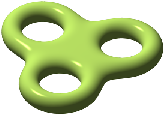
\includegraphics[scale=1.25]{main/Fig02-RiemannSurface}}
\vskip-15pt
\caption{A Riemann surface of genus 3.
}
\label{RiemannSurface}
\end{figure}


\begin{fact}[(Hodge theory)]
The sole topological invariant of a smooth projective curve $C$,
viewed as an analytic space, is its genus. As a manifold it is a
compact, oriented surface, and its genus is half the rank of its first
singular cohomology, $H^{1}(C; \CC)$, which is equal to its first 
de Rham 
cohomology.
Breaking up the de Rham cohomology of any smooth projective complex variety $X$ in terms of holomorphic and antiholomorphic differential
forms we get the \emph{Hodge decomposition}
$$
H^i(X,\CC) = H^i_{\mathrm{de\,Rham}}(X) = 
\tsty\bigoplus\limits_{j=0}^i H^j(\mwedge^{i-j} \Omega_X).
$$
For a smooth curve $C$, this says in  particular that
$$
H^1(C; \CC) = H^0(\omega_C)\oplus H^1(\sO_C) = H^0(\omega_C)\oplus (H^0(\omega_C))^\vee, 
$$
so $ h^0(\omega_C)$ is half the rank of the middle singular cohomology
group, justifying the name ``genus''. For details, 
see~\cite[p.\,116]{Griffiths-Harris1978}.
\end{fact}

A divisor $E$
of negative degree 
satisfies the equation
$H^0(E) = 0$,
so we get the form of the Riemann--Roch theorem
originally proved by 
Riemann:
\index{Riemann, Georg Friedrich Bernhard}%

\begin{corollary}\label{nonspecial RR}
For any divisor $D$ of degree $d$ we have
$$
h^0(D) \geq d - g + 1,
$$
with equality if $d > 2g-2$.
\unif
\end{corollary}

It was 
Gustav Roch,
\index{Roch, Gustav}%
a student of
Riemann's, 
who supplied the correction term $h^0(K_C - D)$ for divisors of lower degree.
The dimension $h^0(K_C-D) = h^1(D)$ was called the 
\emph{superabundance}
\index{superabundance}%
of $D$: the ``expected'' number of sections was $d-g+1$, and $h^1(\cL)$ reflected how much larger the actual number was.

Corollary~\ref{nonspecial RR} and Proposition~\ref{very ample} together show that all high degree divisors come from hyperplane sections in 
suitable embeddings; and unlike the general vanishing theorems, they give a bound on the degree necessary for vanishing
of cohomology and for
global generation:

\begin{corollary}\label{degree 2g+1 embedding}
Let $D$ be a divisor of degree $d$ on a smooth, connected projective curve of genus $g$.
\begin{enumerate}
 \item If $d>2g-2$ then $H^1(\sO_C(D)) = 0$.
 \item If $d \geq 2g$ then $\sO_C(D)$ is generated by global sections; that is, the complete linear series $|D|$ is basepoint free; and $\sO_C(D)$ is very ample unless $D = K_{C}+E$ for some divisor $E$ of degree 2.
 \item If $d \geq 2g+1$ then $\sO_C(D)$ is very ample; that is, the associated morphism $\phi_D : C \to \PP^{d-g}$ is an embedding, and
$D$ is the preimage of the intersection of $C$ with a hyperplane in $ \PP^{d-g}$.
\unif
\end{enumerate}
\end{corollary}

\begin{proof}
If $d>2g-2$ then $K-D$ has negative degree, and thus 
$$h^1(D) = h^0(K-D) = 0. $$ 
\scalebox{0.99}[1]{\hbox spread -9pt{%
The last two parts follow
from the Riemann--Roch theorem and Proposition\,\ref{very ample}.
\unskip}}
\end{proof}

Since the complement of a hyperplane in projective space is an affine space, we get an affine embedding result too:

\begin{corollary}
 If $C$ is any smooth projective curve and $\Gamma \subset C$ a nonempty finite subset then $C \setminus \Gamma$ is affine (that
 is, isomorphic to a closed subscheme of an affine space).
\unif
\end{corollary}

\begin{proof}
Let $D$ be the divisor defined by $\Gamma$. By Corollary~\ref{degree 2g+1 embedding} a high multiple of $D$ is very ample,
and gives an embedding $\phi: C\to \PP^n$ such that the preimage of the intersection of $C$ with some hyperplane $H$
is a multiple of $D$. It follows that $C\setminus \Gamma$ is embedded in $\AA^n = \PP^n\setminus H$.
\end{proof}
 
We can  use Corollary~\ref{nonspecial RR} to determine the Hilbert polynomial of a projective curve. To do this, let $C \subset \PP^r$ be a smooth curve of degree $d$ and genus $g$, and consider the exact sequence of sheaves
$$
0 \to \cI_{C/\PP^r}(m) \to \cO_{\PP^r}(m) \to \cO_C(m) \to 0
$$
and the corresponding exact sequence
$$
 H^0(\cO_{\PP^r}(m)) \ruto{\rho_m} H^0(\cO_C(m)) \to H^1(\cI_{C/\PP^r}(m)) \to 0.
$$
The \emph{Hilbert function} $h_C(m)$ of $C$  is defined in terms of the
\index{Hilbert function}%
homogeneous coordinate ring $R_{C}$ of $C$ by
$$
h_C(m) = \dim_{\CC} (R_{C})_{m} = \rank \rho_m,
$$
where $(R_{C})_{m}$ is the degree $m$ component of the homogeneous coordinate ring of $C$ in $\PP^n` `$.

By Theorem~\ref{Serre--Grothendieck vanishing} we have
$H^1(\cI_{C/\PP^r}(m)) = 0$ for large $m$ so, for large $m$,
$h_{C}(m) =  h^0(\cO_C(m))$. Using 
Theorem~\ref{Serre--Grothendieck vanishing} again, we see that, for large $m$, 
$$
h^0(\cO_C(m)) = \chi(\cO_C(m)).
$$
Finally, by the Riemann--Roch theorem,
$$
\chi (\sO_{C}(m)) = dm-g+1,
$$ 
so, for large $m$, the Hilbert function $h_{C}(m) = dm-g+1$ is in agreement
with the Hilbert polynomial $p_{C}(m) \colonequals \chi(\cO_{C}(m))$.

More generally, we define the \emph{arithmetic genus} and \emph{geometric genus} as follows:
\index{arithmetic genus}%
\index{genus!arithmetic}%
\index{geometric genus}%
\index{genus!geometric}%

\begin{definition}\label{genus Hilbert}\label{pa}\label{genus formula}
If $C\subset \PP^n$ is a 1-dimensional projective scheme with Hilbert polynomial
$p_C(m) = \chi(\sO_C(m))$, the \emph{arithmetic genus} $p_a(C)$ 
of $C$ is $1-\chi(\sO_{C})=1-p_C(0)$. If $C$ is reduced and irreducible, then
\index{geometric genus}%
\index{genus!geometric}%
the \emph{geometric genus} $g(C)$ is the genus of the normalization of $C$.
\end{definition}

We see from the Riemann--Roch theorem that if $C$ is smooth and connected, then $p_a(C) = g(C) = h^0(\omega_C)$, the genus of $C$. We
will see that for reduced and irreducible curves $p_a(C) \geq g(C)$, with equality only when $C$ is smooth.
  For some examples with curves that are not
reduced and irreducible, see Exercise~\ref{pa example}.
  

The Riemann--Roch theorem and Serre duality have extensions to arbitrary coherent sheaves in place of invertible sheaves 
and to singular curves, which we will explain in Chapter~\ref{LinkageChapter}.

Divisors $D$ for which $h^0(K_C - D)>0$ are called \emph{special divisors}. The existence or nonexistence of divisors $D$ with given $h^{0}(D)$ and $h^{1}(D)$ often serves to distinguish one curve from another, and will be an important part of our study.

\subsection*{Residues} 

The 
Rie\-mann--Roch theorem is so central to the study of curves that it is worth understanding from another point
of view.
We remarked at the beginning of Chapter~\ref{linear series} that a
smooth projective curve over $\CC$ is the same thing as a compact
Riemann surface. 
We will briefly adopt
the complex analytic viewpoint, and give an explanation of 
\index{complex analytic viewpoint}%
a special case of Theorem~\ref{RR theorem}.

If $D = \sum a_ip_i$ is an effective divisor 
on a compact Riemann surface $X$ then we write $L(D)$ 
for the vector space of meromorphic functions on $X$ with poles of order 
at most $a_i$ at $p_i$. 

\begin{theorem}
Let $X$ be a compact Riemann surface of genus $g$, and let $D$ be an effective divisor of degree $d$ on $X$. Suppose that $K-D$ is also effective for some canonical divisor $K$.
The dimension of  $L(D)$ is
$d-g+1+\dim_\CC L(K-D)$.
\unif
\end{theorem}

Because  meromorphic functions on a Riemann surface are rational functions on the corresponding
algebraic curve, and $L(D) = H^0(\sO_C(D))$, the assertion is equivalent to Theorem~\ref{RR theorem}.

\begin{proof}
Recall that the 
\emph{residue}
of a meromorphic 1-form $\phi$ at a
\index{residue}%
point $p$ on $X$ is defined by an integral: choose a disc $\Delta \subset X$ containing $p$ and in which $\phi$ is holomorphic except
for its pole at $p$. The residue $\Res_p(\phi)$ is $\sfrac{1}{2\pi i}$
times the integral of $\phi$ along the boundary of $\Delta$. If $z$ is
a local coordinate on $\Delta$ zero at $p$ and we write the
differential $\phi$ as
{\meshing
$$
\phi = \sum_{i=-n}^\infty \!a_iz^i \,dz
$$
then by Cauchy's formula, the residue of $\phi$ at $p$ is the coefficient $a_{-1}$. 
}

\begin{proposition}\label{residue sum}
 If $\phi$ is a meromorphic differential on a compact Riemann surface $X$, then the sum of the residues of $\phi$
 at all the poles of $\phi$ is $0$.
\unif
 \end{proposition}
 
\begin{proof}
Apply 
Stokes' theorem
\index{Stokes' theorem}%
to the complement of the union of small discs around each of the poles of $\phi$.
\end{proof}

Let  $D = \sum a_ip_i$ be an effective divisor on $X$, and set $d = \sum a_i = \deg D$. Locally, a function with a pole of order at most $n$ at $p$ may be written in terms of a local coordinate $z$ at $p$ as $\sum_{i=-n}^\infty a_{i}z^{i} $;
the sum $\sum_{i=-n}^{-1} a_{i}z^{i}$ is called its \emph{polar part}.
By the maximum principle, a meromorphic function in $L(D)$ is determined, up to the addition of a constant, by its polar parts at the points~$p_i$. Thus we have $\dim L(D) \leq d+1$.
{\meshing\par}

When is a given collection $c_1,\dots,c_d \in \CC[z^{-1}]$ the polar parts of a global meromorphic function $f$ on $X$? A necessary condition
is that if $\phi \in L(K)$ is a holomorphic differential on $X$, then
$$
\sum \Res_{p_i}(f \cdot \phi) = 0.
$$
This gives $g$ linear relations on the $c_i$. However, if $\phi$ is a holomorphic differential vanishing at all the points $p_i$
then the corresponding relation is trivial. Thus the number of linearly independent relations on the polar parts of $f$ is actually $g - \dim L(K-D)$; and we arrive at an inequality
$$
\dim L(D) \leq d + 1 - g + \dim L(K-D).
$$

This is a priori only an inequality. But we can apply the same logic to an effective divisor $K-D$, and we see that
\begin{align*}
\dim L(K-D) &\leq \deg(K-D) + 1 - g + L(K - (K-D)) \\
& = 2g - 2 - d + 1 - g  + L(D) \\
&= g - d - 1 + L(D).
\end{align*}
Adding the two inequalities we have
$$
L(D) + L(K-D) \leq L(D) + L(K-D).
$$
Since the sum of the inequalities is an equality, we conclude that each inequality is also an equality; this is the Riemann--Roch formula
in our special case.
\end{proof}

\subsection*{Arithmetic genus and geometric genus}

Throughout this book, we will be primarily concerned with the geometry of smooth curves. Of course singular curves will arise\emdash for example, as images of smooth curves under morphisms that are not embeddings. At least when $C$ is a 1-dimensional variety (that is, a 
reduced irreducible 1-dimensional scheme) we can  regard $C$ as the image of a smooth curve in an optimal way:

\begin{proposition}\label{resolution of singularities}
If $C_0$ is a projective variety of dimension 1 then the \emph{normalization} $\nu: C \to C_0$ of $C_0$ is a birational
morphism from a smooth curve $C$. The curve $C$ is again projective, and the pair $(C, \nu)$ is
unique up to  isomorphism. In particular, every birational map of smooth curves is an isomorphism.
\unif
\end{proposition}
 
\begin{proof}
  We use the result that the normalization ($=$ integral closure) of a domain
finitely generated over a field is again finitely generated, and nonsingular in codimension 1 \cite[Theorem 4.14 and 11.5]{Eisenbud1995}. Thus,
starting with a projective embedding of $C$ we normalize the homogeneous coordinate ring of $C$. The resulting ring
may have generators in many degrees, but a suitable Veronese subring will be generated in a single degree, and thus
is the homogeneous coordinate ring of a smooth projective curve. 

Localization
commutes with normalization, and any map from a normal ring to a
domain factors uniquely through any normalization. 
Therefore
the normalization constructed above is independent of the choices.
\end{proof}

A different procedure for finding a smooth curve birational to a given curve
is explained in 
Exercises \ref{Veronese of plane curve} to \ref{Mumford resolution argument}.


Still assuming that $C_0$ is reduced and irreducible, we can relate
\index{arithmetic genus}%
\index{geometric genus}%
\index{genus!arithmetic versus geometric}%
the
arithmetic and geometric genera
of $C_0$ using the map of sheaves
$$
\cO_{C_0} \to \nu_*\cO_C.
$$
Since the normalization map of rings  is injective and finite, this map is injective. The cokernel $\sF$ is a coherent sheaf supported on the singular points of $C_0$, and is thus finite over $\CC$. 
The definition implies that there is a short exact sequence
$$
0 \to \cO_{C_0} \to \nu_*\cO_C \to \cF \to 0.
$$

\begin{proposition}\label{pa and delta}
Suppose that $C_{0}$ is a reduced, irreducible curve and let  $\nu: C\to C_{0}$ be its normalization.
Let $\sF = \nu_{*}\sO_{C}/\sO_{C_{0}}$. If we set 
$\delta(C_{0}) \colonequals h^{0}(\sF)$, 
then
 $$
p_a(C_0) - g(C) =  \delta(C_{0})
$$ 
\end{proposition}

\begin{proof}
 Since the normalization map $\nu: C \to C_0$ is finite,  the direct images $R^i\nu_*\cO_C$ vanish for $i > 0$, 
so the Leray spectral sequence 
(see \ref{Leray} just below)
computes $\chi(\nu_*\cO_C) = \chi(\cO_C)$. Thus
$$
p_a(C_0) - g(C) =  \chi(\cO_{C}) -   \chi(\cO_{C_0}) = \chi(\cF) = h^0(\cF) 
$$ 
since the support of $\cF$ is finite.
\end{proof}

The operation of normalization localizes, so we can understand $\sF$ by looking at it locally.
Writing $R$ for the affine ring of some affine subset $U\subset C_{0}$ we see that $\sO_{C}|_{U}$
is the integral closure $\ovR$ of $R$, so $\sF|_{U}$ is $\ovR/R$. Thus
the annihilator of $\sF|_{U}$, called the \emph{conductor}
$\ff_{\ovR/R}$,
is an ideal of both $\ovR$ and $R$,
and correspondingly $\nu^{-1}(\ff_{C/C_{0}})$ 
is also an ideal sheaf in $\sO_{C}$.

Informally, we may say that $\delta(C_{0})$ is the number of linear
conditions a locally defined function $f$ on $C$ has to satisfy to be
the pullback of a function from $C_0$. The length of the stalk of
$\cF$ at a particular singular point $p \in C_0$ is called the
\index{delta invariant@$\delta$ invariant}%
\emph{$\delta$ invariant} $\delta_p$ of the singularity. Thus 
$$
p_a(C_0) - g(C) = \sum_{p @\in@ (C_0)_{\mathrm{sing}}\!\!} \delta_p.
$$ 

\begin{fact}~\label{Leray}
 In general, the 
Leray spectral sequence
\index{Leray spectral sequence}%
addresses the situation of  a morphism $f:X\to Y$ of varieties or schemes, 
 and a coherent sheaf $\sG$  on the source $X$; it says in this circumstance that there is a spectral sequence
  $$
  \HH^p(R^qf_*(\sG)) \Longrightarrow \HH^{p+q}(\sG).
  $$
(This is a special case of the spectral sequence for the derived functors of a composite functor ($H^0$ composed with $f_*$);
see~\cite[II.4.17.1]{Godement} or \cite[Section III.7]{Gelfand-Manin} for proofs.)
\end{fact}

In the simplest cases the $\delta$ invariant is easy to compute:


\begin{enumerate}

\item A 
\index{node}%
\emph{node}
of a curve $C_0$ is a point $p$ such that
  an analytic neighborhood of $p$ in $C_0$ consists of two smooth arcs
  intersecting transversely at $p$ 
(See Figure \ref{simplesing}, left.)
Equivalently, the completion of
  the local ring $\cO_{C_0,p}$ is isomorphic to $k\[x,y\]/(xy)$. If $p
  \in C_0$ is a node, its preimage in the normalization $C$ of $C_0$
  consists of two points $r,s\in C$. The condition for a function $f$
  on $C$ to descend to $C_0$\emdash that is, to be the pullback of a function
on $C_0$\emdash is  that $f(r)=f(s)$; this is one 
linear condition, so $\delta_p = 1$.

\item  
A
\index{cusp}%
\emph{cusp}
of a curve $C_0$ is a point $p$
  such that an analytic neighborhood of $p$ in $C_0$ is given by the
  equation $y^2=x^3` `$. 
(See Figure \ref{simplesing}, second from left.)
If $p \in C_0$ is a cusp then its
  preimage in the normalization $C$ of $C_0$ will consist of one point
  $r\in C$. The condition for a function $f$ on $C$  is that the
  derivative $f'(r)=0$; again, this is one linear condition, so
  $\delta_p = 1$. 
\end{enumerate}

We will give more examples at the end of
Chapter~\ref{PlaneCurvesChapter}.



\begin{figure}   % appears as 2.4
\centerline{%
  \includegraphics[height=2in]{"main/Fig02-sing-node"}\hfil\quad
  \includegraphics[height=2in]{"main/Fig02-sing-cusp"}\hfil\quad
  \includegraphics[height=2in]{"main/Fig02-sing-tacnode"}\hfil\quad
  \includegraphics[height=2in]{"main/Fig02-sing-triple"}}
\caption{Simple planar curve singularities.
\index{tacnode}%
\index{triple point}%
\index{plane curve!singularities}%
\index{singularity!of planar curve}%
\label{simplesing}
}
\end{figure}


\section{The canonical morphism}

We now return to the world of smooth curves.
\index{canonical morphism}\index{morphism!canonical}%

 The canonical sheaf on $\PP^1$ has negative degree, so $|K_{\PP^1}| = \emptyset$. If $C$ is a curve
 of genus $1$ then the canonical sheaf     has a nonzero global section, and since the sheaf has degree $2g-2=0$ this is nowhere vanishing, whence
 $\omega_C = \sO_C$, and $K_C = 0$. Thus in studying the canonical series we restrict our attention to curves $C$ of genus $g\geq 2$. 
 
 \begin{theorem}\label{canonical series is very ample} Let $C$ be a smooth curve of genus $\geq 2$.
\begin{enumerate}
 \item $|K_C|$ is basepoint free.
 \item $|K_C|$ is very ample if and only if $C$ admits no map of degree 2 to $\PP^1` `$.
\unif
\end{enumerate}
\end{theorem}

A curve of genus $\geq 2$
is said to be \emph{hyperelliptic} if there exists a 
morphism
$f: C \to \PP^1$ 
of degree 2.
\index{hyperelliptic}%
\index{morphism!of degree 2}%
It is easy to describe this in terms of linear series:

\begin{lemma}\label{deg 2 morphism}
Let $C$ be a smooth, projective curve of genus $g\geq 2$. If $C$ has an invertible sheaf $\cL$ of degree $\leq 2$ with two independent sections, then $\cL$ has degree~$2$ and
$|\cL|$ defines a morphism of degree $2$ to $\PP^{1}$, so $C$ is
hyperelliptic. In particular, if $g(C) = 2$ then the canonical series
$|K_{C}|$ defines a $2$-to-$1$ morphism to $\PP^{1}$, so $C$ is
hyperelliptic.
\unif
\end{lemma}

\begin{proof}
Since $C \not\cong \PP^1` `$,  Theorem~\ref{characterization of P1} shows that $C$ cannot have a 1-dimensional linear series
of degree $< 2$. Thus $\sL$ has degree exactly 2, and no 
basepoints,
so it defines a morphism of degree 2 to $\PP^1$ as claimed.
\end{proof}

\begin{proof}[Proof of Theorem~\ref{canonical series is very ample}]
A point $p$ is a basepoint of $|K_C|$ if and only if 
$$h^0(K_C-p) = h^0(K_C) = g.$$ 
By the Riemann--Roch theorem,
this is equivalent to $h^0(p) =2$, which would imply that $C\cong \PP^1$ by Theorem~\ref{characterization of P1}. Thus $K_C$
has no basepoints.

By Proposition~\ref{very ample} we 
must
show that for any 
two
points $p, q \in C$ we have
$$
h^0(K_C(-p-q)) = h^0(K_C)-2 = g-2.
$$
Applying the Riemann--Roch theorem we see 
that this fails if and only if $h^0(\cO_C(p+q)) \geq 2$ for some $p,q
\in C$. By Lemma~\ref{deg 2 morphism}, this implies that $C$ is
hyperelliptic. Conversely, if $C$ is hyperelliptic then for some
divisor $D = p+q$ we have $h^0(D) = 2$, whence $h^0(K-p-q) = h^0(K)
-1$ by 
the Riemann--Roch formula.
\emergencystretch5.5pt
\end{proof}

The image of the canonical morphism of a nonhyperelliptic curve of
genus $g>2$ is called a 
\emph{canonical curve},
\index{canonical curve}%
and (for a nonhyperelliptic curve) we  
speak of the image as being \emph{canonically embedded}.


\subsection*{Geometric Riemann--Roch}

There is a useful way of expressing the Riemann--Roch formula in terms
of the geometry of the canonical map. Suppose $C \subset \PP^r$ is a
smooth curve and $D$ an effective divisor on $C$, thought of as a
subscheme of $C$. We define the 
\emph{span}
\index{span!of effective divisor}%
$\ovD$ of $D$ to be the
intersection of the hyperplanes $H \subset \PP^r$ containing $D$. More
generally, if $\phi : C \to \PP^r$ is a map and $D$ an effective
divisor on $C$, we define the span $\overline{\phi(D)} \subset \PP^r$
to be the intersection 
$$
\overline{\phi(D)} \colonequals \bigcap_{ 
\substack{H \subset \PP^r \text{ a hyperplane} \\D \subset
  \phi^{-1}(H)}}
H.
$$

Now suppose $C$ is a smooth curve of genus $g\geq 2$ and $\phi_K: C\to \PP^{g-1}$ is the canonical morphism.
If  $D$ is an effective divisor on $C$ of degree $d$, then since the hyperplanes in $\PP^{g-1}$ containing $\phi_K(D)$ correspond (up to scalars) to sections of $K_C$ vanishing on $D$, we see that
$$
h^0(K_C-D) = \codim \overline{ \phi_K(D)} \subset \PP^{g-1}= g - 1 - \dim \overline{ \phi_K(D)}.
$$
\index{geometric!Riemann--Roch theorem}%
\index{Riemann--Roch theorem!geometric}%
Applying the Riemann--Roch theorem we obtain  the \emph{geometric Riemann--Roch theorem}:

\begin{corollary}\label{geometric RR}
If $D$ is a divisor on a smooth curve $C$ of genus $\geq 2$ then
$$
r(D) = d - 1 - \dim \overline{ \phi_K(D)}.
\vspace*{-3pt}
$$
\end{corollary}
%
In particular, if $D = \sum_{i=1}^dp_i$ is a sum of distinct points, then
 the dimension of the linear series $|D|$  is equal to the number of linear relations among the images of the $p_i$ on the canonical 
 image of $C$. 
 Thus, for example, a divisor given as the sum $D = p+q+r$ of three
 points will move in a pencil if and only if the three points are
 collinear on the canonical model. 

In general, 
the condition that a form of degree $d$ vanishes at 
a given point $p$ in $\PP^r$ is expressed
by one homogeneous linear
equation on the coefficients of the form, obtained by evaluating the variables at 
 the coordinates of $p$.  Thus the condition of vanishing on a set $\Gamma$ of $\gamma$ points is given by
 $\gamma$ linear equations and the same is true when $\Gamma$ is a finite subscheme
 of length $\gamma$, as one sees from the exact sequence
 $$
 0\to H^0(\sI_\Gamma(d)) \to H^0(\sO_{\PP^r}(d)) \ruto{ev} H^0(\sO_{\Gamma}(d)) \to 0,
 $$
 bearing in mind that 
 $$
 H^0(\sO_{\Gamma}(d)) \cong H^0(\sO_{\Gamma}) \cong \CC^\gamma.
 $$
However, the linear equations may be dependent; that is, the map marked $ev$
above may have rank $<\gamma$. We will say that the points of $\Gamma$
\emph{fail to impose independent conditions on hypersurfaces of degree $d$}
by the amount equal to $\gamma - \rank(ev)$. 

With this terminology, the geometric Riemann--Roch theorem says that 
the dimension of the complete linear series $|D|$ on a smooth curve $C$
is the amount by which the points of $D$ fail to impose independent conditions
on canonical divisors, and the geometric version simply translates this into 
 hyperplanes in the canonical embedding of $C$. 
\index{Cayley--Bacharach--Macaulay theorem}%
The Cayley--Bacharach--Macaulay
theorem~\ref{CBM} 
is a useful
special case.

\begin{remark}
For a singular curve $C_0$ to have a canonical morphism it is necessary first of all that its canonical sheaf
 $\omega_{C_0}$ be invertible; when this is the case, we say that $C_0$ is (locally) Gorenstein, and then
\index{locally Gorenstein}%
\index{Gorenstein!locally}%
the theory above can be applied. See for example \cite{graphcurves} and \cite{ribbons} for examples. 
\end{remark}

\subsection*{Linear series on a hyperelliptic curve}
We can describe the canonical map of a hyperelliptic curve\emdash and indeed all its special linear series\emdash quite precisely:

\begin{corollary}\label{canonical on hyperelliptic}
Let $C$ be a smooth hyperelliptic curve of genus $g\geq 2$. The curve $C$ admits a unique degree 2 morphism $\pi: C\to \PP^1` `$,
and the canonical map $\phi_K: C\to \PP^{g-1}$ is the composition of $\pi$ with the Veronese map of degree $g-1$ from
\index{Veronese!map}%
$\PP^1$ to the rational normal curve of degree $g-1$; in particular, every canonical divisor is a sum of $g-1$ fibers of $\pi$ and vice versa.
\unif
\end{corollary}

\begin{proof}
If $D$ is a general fiber of a degree 2 map $\pi:C\to \PP^1$ so that $D= p+q$ and $r(D) = 1$, then by the Riemann--Roch theorem or its geometric version, $D$ imposes only one condition on sections of $K_C$; that is, $\phi_K(p) = \phi_K(q)$. Consequently the degree of the canonical morphism $\phi_K$ is at least 2, and the image is thus a nondegenerate curve in $\PP^{g-1}$ of degree $\leq (2g-2)/2 = g-1$. By Theorem~\ref{characterization of P1}, the image of $\phi_K$ is the rational normal curve of degree $g-1$ and every fiber of $\phi_K$ is a divisor linearly equivalent to $D$. It follows that $\pi$ is determined by $K$, so it is unique. Since every canonical divisor is the pullback of a hyperplane section of the rational normal curve,
every canonical divisor is a sum of $g-1$ fibers of $\pi$.
\end{proof}

We can use these ideas to analyze all special divisors.
\index{special divisor}%
\index{divisor!special}%

\begin{corollary}\label{special on hyperelliptic} Let $C$ be a smooth 
hyperelliptic curve
\index{hyperelliptic curve}%
with map $\pi: C\to \PP^1$ of degree 2.
Every special divisor $D$ of degree $d$ on 
$C$ is a sum of $s$ fibers of $\pi$ and $d-2s$ points
$p_1,\dots,p_{d-2s}$ with distinct images under the canonical map; and
in this case we have $r(D) = s$ and the points $p_i$ are basepoints
of the linear series $|D|$.
Thus
no divisor on a hyperelliptic curve is both special and very ample.
\unif
\end{corollary}

\begin{proof}
Suppose that $D$ contains the sum $E$ of $s$ fibers of $\pi$ and no more; and write $D = E+D'$, with $\deg D' = d-2s$.
 
If $\phi_K:C \to \PP^{g-1}$ is the canonical map, then $\phi_K(D')$ consists of $d-2s$ distinct points, while $\phi_K(E)$ consists of
$s$ points. By Corollary~\ref{independence of points on a RNC} the span of $\phi_K(D)$ has dimension $\min\{g-1, d-s-1\}$, so 
$r(D) = d-1-\min\{g-1, d-s-1\} = \max \{s,d-g\}$. Since $D$ is a special divisor, $r(D) > d-g$, so $r(D) = s$. 
Since $r(E) =s$, we see that $E$ is basepoint free, so $D'$ is the base locus of $D$.
\end{proof}

\section{Clifford's theorem}\label{Clifford Section}

While the Riemann--Roch theorem gives a lower bound for the dimension of a linear series, $r(\sL) \colonequals h^0(\sL)-1 \geq \deg \sL -g$, Clifford's theorem
\index{Clifford's theorem}%
gives an upper bound. If $\deg \sL>2g-2$, then the Riemann--Roch
inequality becomes an equality, so it is enough to treat the case
$\deg \sL \leq 2g-2$. The bound is actually a corollary of the 
Riemann--Roch theorem.

\begin{corollary}\label{Clifford bound}
 Let $C$ be a curve of genus $g$ and $\cL$ an invertible sheaf of degree $d \leq 2g-2$. Then
$$
r(\cL) \leq \frac{d}{2}.
$$
\end{corollary}

\begin{proof}
If $\cL$ is nonspecial then, since $g\geq d/2 + 1$, we have $r(\cL) = d-g+1\leq d/2$.
Otherwise we have
$$
r(K_C\otimes \cL^{-1}) = r(\cL) +g - d - 1
$$
by the Riemann--Roch theorem,
and so by Proposition~\ref{sum of linear series}
$$
g = r(K_C)+1  \geq r(\cL) + r(K_C\otimes \cL^{-1}) +1  = 2r(\cL) +g - d;
$$
hence $r(\cL) \leq d/2$.
\end{proof}

The usual statement of Clifford's theorem includes a description of when equality can occur:

\begin{theorem}\label{Clifford}\label{Clifford equality}
Let $C$ be a curve of genus $g$ and $\cL$ an invertible sheaf of degree $d \leq 2g-2$. If
$$
r(\cL) = \frac{d}{2},
$$
the largest possible value, then either
\begin{enumerate}
\item $d=0$ and $\cL = \cO_C@$;
\item $d = 2g-2$ and $\cL = K_C@$; or
\item $C$ is hyperelliptic, and $|\cL|$ is a multiple of the $g^1_2$ on $C$.
\unif
\end{enumerate}
\end{theorem}

From Corollary~\ref{canonical on hyperelliptic} and Corollary~\ref{geometric RR} we see that the equality does indeed hold
in each of the cases enumerated. See
Corollary~\ref{equality in Clifford from Martens} for the converse and \cite[IV.5.4]{Hartshorne1977}
for a different proof.

 \section{Curves on surfaces}\label{surface basics}
 
 We will often analyze curves  on a smooth surface. Compared to the theory of linear series on curves, there is a new element: the intersection pairing. We refer to~\cite[Chapter V]{Hartshorne1977}
\index{intersection pairing}%
 and~\cite[Chapter I]{Beauville} for 
proofs
of the unproven statements in this section.
 We suppose for this section that $S$ is a smooth projective surface,
 and write $\Pic(S)$ for the group of invertible sheaves on $S$.

\subsection*{The intersection pairing}

When two codimension 1 subschemes $D,E$ on $S$ 
meet transversely we define $D\cdot E$ to be the number of points in which they meet.  
It is less obvious how one might define an intersection number $D\cdot E$ in more general cases,
including the case $D=E$. However 
a codimension 1 subvariety of $S$ has a 
\index{fundamental class}%
fundamental class in $H^{2}(X,\ZZ)$, and the product just defined
agrees with the cup product pairing
\index{cup product pairing}%
$$
H^{2}(S,\ZZ) \times H^{2}(S,\ZZ) \to H^4(S,\ZZ)\cong \ZZ,
$$
showing that it is possible. For example, the self-intersection $D\cdot D$ can be realized geometrically
 by choosing a normal vector field $\sigma$ on $D$ and using it to push a copy $D'$ of $D$ infinitesimally away from $D$; then
 one can count the points where $\sigma$ vanishes (see Figure~\ref{vanishing of normal vector field}. Here one must take orientations into account,
 and the result is that $D\cdot D$ may be negative. In the previous case (and when $\sigma$ is complex analytic)
 the multiplicities are all positive because a complex subvariety is canonically oriented using the orientation of $\CC$
 itself.

\begin{figure}   % appears as 2.5
\Small
\centerline{\includegraphics[height=1.75in]{"main/Fig02-strip"}%
\llap{\raise56pt\hbox{$D$}\hskip29pt}%
\llap{\raise72pt\hbox{$D'$}\hskip40pt}%
}
\captionPlus{Fig02-strip}{The result, $D'$, of moving $D$ infinitesimally along a normal vector field meets $D$ twice.}
\label{vanishing of normal vector field}
\end{figure}

This pairing can be realized algebraically as follows:

First, if $D$ and $E$ have no common
\index{intersection multiplicity}%
components, then the \emph{intersection multiplicity} 
$\mathrm{mult}_{p}(D,E)$ at $p\in S$
\index{mult@$\mathrm{mult}_p$}%
is defined as the vector space dimension of the local ring $\sO_{S,p}/(\sI_{D,p}+\sI_{E,p})$, and 
$$
D\cdot E = \sum_p \mathrm{mult}_{p}(D,E).
$$

Quite generally, 
the intersection product can be computed using the (algebraic) Euler
characteristic. 
This
works even for 
Cartier divisors
on a singular surface: Setting $\sL \colonequals \sO_S(D)$ and
\index{Euler characteristic}%
\index{Cartier divisor}%
$\sM \colonequals \sO_S(E)$ to simplify the notation, we have 
$$
D\cdot E = \chi(\sO_S)-\chi(\sL^{-1}) -\chi(\sM^{-1}) +\chi(\sL^{-1}\otimes \sM^{-1}) 
.
$$

\begin{theorem} The pairing $(D,E) \mapsto (D\cdot E)$ is the unique bilinear map
$\Pic(S) \times \Pic(S) \to \ZZ$ extending the case of intersections of two curves meeting transversely at smooth points of $S$. 
\unif
\end{theorem}

An important special case is that of the self-intersection $D\cdot D = D^2` `$. The general formula reduces immediately to the case of an effective divisor, and in that case it resembles the $C^{\infty}$ construction above:

\begin{corollary}\label{self-intersection number}
If $D$ is a codimension $1$ subscheme of $S$, then the self-intersection $D\cdot D$ is the degree of the normal bundle
$\sN_{D/S} \colonequals \sO_{D}(D)$.
\unif
\end{corollary}

\begin{proof}
Substituting $\sO_{S}(-D)$ for both $\sL^{-1}$ and $\sM^{-1}$ we
have the
exact sequences
\begin{align*}
 0\to \sO_{S}(-D)\to &\; \sO_{S}\to \sO_{D}\to 0,\\
0\to \sO_{S}(-2D)\to &\; \sO_{S}(-D)\to \sO_{D}(-D)\to 0;
\end{align*}
the Riemann--Roch theorem 
then gives
\begin{align*}
\chi(\sO_{S}) -\chi(\sO_{S}(-D)) &= \chi(\sO_{D}) = -p_{a}(D) +1,\\
\chi(\sO_{S}(-D)) -\chi(\sO_{S}(-2D)) &= \chi(\sO_{D}(-D)) = -\deg \sO_{D}(D) - p_{a}(D) +1.
\end{align*}
Subtracting the second of these equations from the first we see that
$D\cdot D = \deg \sO_{D}(D)$.
\end{proof}

Using the intersection pairing we can turn the adjunction formula of Proposition~\ref{adjunction} into a numerical formula:

\begin{theorem}[adjunction formula]\label{adjunction formula} 
If $C$ is a Cartier divisor on a smooth surface $S$ then
\index{adjunction formula}%
$$
p_a(C) = \frac{(K_X+C)\cdot C}{2} +1.
 $$
\end{theorem}

\subsection*{The Riemann--Roch theorem for smooth surfaces}
Often we wish to compute the dimension of the space of sections of an invertible sheaf, but
as with the case of curves, the Euler characteristic is more accessible:

\begin{theorem}[Riemann--Roch for surfaces] Let $\sL$ be an invertible sheaf on a smooth surface $S$.
\index{Riemann--Roch theorem!for surfaces}%
\index{Euler characteristic}%
The Euler characteristic $\chi(D) \colonequals h^0(\sL)-h^1(\sL)+h^2(\sL)$, where $\sL = \sO_S(D)$, is given by
$$
\chi(D) = \chi(\sO_S) + \frac{(D-K_S)\cdot D}{2}+1
.
$$
\end{theorem}

\subsection*{Blowups of smooth surfaces}

It is useful to know what happens under mappings of surfaces, particularly the case of the mapping
\index{blowup!of smooth surface}%
corresponding to blowing up a point.

\begin{theorem}\label{divisor classes on blowup}
If $\pi: X \to Y$ is a birational map of smooth surfaces, then the pullback map on divisors
preserves the intersection pairing. If $X$ is the blowup of~$Y$ at a point $p$ with exceptional
divisor $E = \pi^{-1}(p)$, then:

\begin{enumerate}
 \item $\Pic X =\pi^*(\Pic Y) \oplus \ZZ E$.
\item The canonical class on $X$ is given by $K_X = \pi^*(K_Y)+E$.
 \item The intersection pairing on $\Pic X$ is given by:
 
\begin{itemize}
\item $\pi^*(D)\cdot\pi^*(D') = D\cdot D'$ for all $D,D'\in \Pic Y$.
\item $\pi^*(D)\cdot E = 0$ for all $D\in \Pic Y$.
 \item $E\cdot E = -1$.
 \item $K_X\cdot E = -1$.
 \item If $C$ is a curve that has an $m$-fold point at $p$ then
   $\pi^{-1}(C)$ contains $E$ with multiplicity $m$, so that the 
\index{proper transform}%
proper transform
 $\tilde C$\emdash that is, the closure in $X$ of the preimage of $C \setminus \{p\}$\emdash has class
 $$
 \tilde C \sim \pi^*C - mE.
 $$
 \end{itemize}
\end{enumerate}
\end{theorem}

Using these facts, we can compare the adjunction formula applied to a curve $C$ on a smooth surface $S$ to the formula applied to the proper transform $\tilde C \subset \tilde S$: we have
$$
\tilde C \cdot \tilde C = C \cdot C - m^2 \quad \text{and} \quad \tilde C \cdot K_{\tilde S} = C \cdot K_S + m.
$$
Combining these, we arrive at the formula
$$
p_a(\tilde C) = p_a(C) - \mbinom{m}{2},
$$
and thus the $\delta$ invariant of $p \in C$ is $\tbinom{m}{2}$ plus the sum of the $\delta$ invariants of all the 
points of $\tilde C$ in the preimage of $p$. One can resolve the curve singularity by repeatedly blowing up in this way and thus compute the $\delta$ invariant
of any singularity as a sum of binomial coefficients.

In the special case where $\tilde C$ is smooth\emdash for example, if
the point $p \in C$ is an (\emph{ordinary}) \emph{$m$-fold point}, consisting
\index{multiple point, $m$-fold point}%
\index{ordinary singularity}%
of $m$ smooth branches with distinct tangent lines\emdash we conclude
that the $\delta$ invariant of the point $p$ is $\tbinom{m}{2}$. 


Blowups occur frequently in the theory of surfaces, and are
\index{Castelnuovo's theorem}%
characterized by \emph{Castelnuovo's theorem} 
\cite[Theorem V.5.7]{Hartshorne1977}. 

\begin{theorem}
If $E\subset X$ is a curve on a smooth projective surface $X$ and
\index{blowdown}%
 that $E^2 = E\cdot K_X = -1$ then $E$ can be ``blown down'' in the sense that
 $X$ is the blowup of a smooth surface $Y$ at a point $p\in Y$, and $E$ is the exceptional divisor.
\end{theorem}




\section{Quadrics in $\PP^3$ and the curves they contain}
\label{Div of quadric}
 
 We will frequently be interested in curves on a quadric surface in $\PP^3` `$, and we can describe these
curves and their intersections very concretely.

\subsection*{The classification of quadrics} The form defining a quadric $Q\subset \PP^{3}$ can be written in suitable
\index{classification of quadrics}\index{quadric!classification of --s}%
coordinates $x_{i}$ as 
$$q = \sum_{i=0}^{3} x_{i}^{2},$$ 
where $r\leq 4$ is the \emph{rank} of $Q$. (The corresponding
statement is also true in $\PP^{r}$, with $m\leq r+1$.) Equivalently, this is the rank of the symmetric matrix $M$
representing the bilinear form $\frac12(q(x+y)-q(x)-q(y))$.

\begin{enumerate}
\item A quadric of rank 1 is a double plane.
\index{double plane}%
\item A quadric of rank 2 is the union of two distinct planes. 
\item A quadric $Q$ of rank 3 is a cone over a smooth plane conic. The cone point is called the vertex. Every line
\index{vertex}%
on such a quadric passes through the vertex. The 
Picard group
\index{Picard group}%
of $Q$ is $\ZZ$
\cite[Exercise II.6.5]{Hartshorne1977}.

\item A quadric $Q$ of rank 4 is smooth and is isomorphic to
  $\PP^{1}\times \PP^{1} \subset \PP^{3}$, embedded by the Segre
  embedding. Every line on such a quadric has the form $\PP^{1}\times
  \{p\}$ or $\{p\} \times \PP^{1}$; the two families of such lines are
  called 
\emph{rulings}.
\unskip
\index{ruling}%
\index{Segre embedding}%
\label{smooth quadric}
The Picard group of $Q$ is $\ZZ\times \ZZ$, generated by the lines of the rulings
\cite[Example II.6.1]{Hartshorne1977}.

\item Quadrics in $\PP^{r}$: Inside the space $\PP(\sO_{\PP^{r}}(2)) = \PP^{\sbinom{r+2}{2}-1}$ the space
of singular quadrics is a hypersurface of degree $r+1$, called the \emph{discriminant}, which is defined by the determinant of a generic symmetric
\index{discriminant}%
$(r+1)\times (r+1)$ matrix $M$. More generally, the rank $k$ locus is defined by the $(k+1)\times (k+1)$
minors of $M$.
\end{enumerate}

%\subsection*{Curves on quadrics}

It follows that
an irreducible nondegenerate  curve cannot be contained in a quadric of rank 1 or 2.

\subsection*{Some classes of curves on quadrics}

\begin{example}\label{curve on rank 3 quadric}
Let $C$ be a reduced curve on a quadric $Q$ of rank 3 in $\PP^{3}$. 
If $C$ has even degree $2m$ then $C$ is a complete intersection
of the quadric with a hypersurface of degree $m$. Therefore if the curve is smooth it cannot contain the vertex of the quadric. The genus of $C$ is $(m-1)^{2}$.

If $C$ has odd degree $2m+1$, then the union of $C$ with a line on the quadric has even degree,
so if $L_{1}, L_{2}$ are lines on the quadric, then 
$$
C\cup L_{1} = Q\cap F_{1} \quad\hbox{and}\quad C\cup L_{2} = Q\cap F_{2}
$$
are complete intersections of $Q$ with forms of degree $m+1$, and the homogeneous ideal of $C$ is generated by the equations
of $Q,F_{1}$ and $F_{2}$. The genus of $C$ is $m(m-1)$. The curve $C$ contains the vertex, and is a 
\index{Weil divisor}%
\index{Cartier divisor}%
Weil divisor, not a Cartier divisor. These things follow from the description of the desingularization
of $Q$ in Corollary~\ref{singular scrolls}.
\end{example}

\begin{example}
\label{curves on quadrics}
If $C$ is a reduced curve on a quadric $Q$ of rank 4, then in terms of the isomorphism
$Q \cong \PP^{1}\times \PP^{1}$ we can express the divisor class of $C$ as $(a,b)\in \Pic(Q) = \ZZ\oplus \ZZ$.
The intersection form on $Q$ is determined by the fact that the lines of a ruling are all linearly equivalent,
so that $(1,0)^{2} = (0,1)^2=0$ and $(1,0)\cdot (0,1) = 1$; thus $(a,b)\cdot (d,e) = ae+bd$. The hyperplane section
has class $(1,1)$, and the canonical class is $(K_{\PP^{3}}+Q)\mid_{Q} = (-2,-2)$ by the adjunction formula. 

Thus
if $C$ has class $(a,b)$ then the degree of $C$ is $a+b$, while the genus of $C$ is $(a-1)(b-1)$. Note that 
if  $a =b$, the curve is a complete intersection, and if $b = a+1$ then the curve is residual to
a line in a complete intersection of the quadric with a surface of degree $b$. In these cases we get the same genus and degree as we would for a curve
on a rank 3 quadric.


The cohomology of $\sO_{Q}(a,b)$ is determined by the K\"unneth formula
\index{K\"unneth formula}%
\index{Leray spectral sequence}%
(or the Leray spectral sequence) as
$$
H^{i}(\sO_{Q}(a,b)) = \tsty\bigoplus\limits_{i = s+t}H^{s}
(\sO_{\PP^{1}}(a))\otimes H^{t}(\sO_{\PP^{1}}(b)).
$$
The degrees of the generators of the homogeneous ideal of $C$ can be determined from the exact sequence
$$
0\to \sI_{Q/\PP^{3}} \to \sI_{C/\PP^{3}} \to \sI_{C/Q} \to 0.
$$
Since $ \sI_{C/Q} (m) = (m-a,m-b)$ we see that, supposing $0<a\leq b$ and $1<b$
there are no generators other than the equation $q$ of $Q$ having degree $<b$, and there are 
$b-a+1$ generators of degree exactly $b$; with $q$ these are the minimal generators of the homogeneous
ideal (Exercise~\ref{curve on rank 4 quadric}).
\end{example}

\section{Exercises}


\begin{exercise}\label{characterization of degree}
\index{degree!of a projective scheme}%
\index{projective scheme!degree of}%
\begin{enumerate}
\item The degree of a zero-dimensional subscheme $X\subset \PP^r$ is by definition the value of the Hilbert polynomial of $X$, which is a constant. Show that
this is the sum of the lengths of the components of $X$. 

\item The degree of a projective subscheme $X\subset \PP^r$ of dimension $n$ is defined to be the degree of the $0$-dimensional scheme
\index{degree!of projective subscheme}%
\index{projective subscheme!degree of}%
that is the intersection of $X$ with a general plane of degree $r-n$. Prove that this is the leading coefficient of the Hilbert polynomial, multiplied
\index{Hilbert polynomial}%
by $n!@$. 

\item If $C\subset \PP^r$ is a smooth curve of genus $g$ and degree
  $d$, show that the 
 Hilbert polynomial of $C$ is $H_C(m) = dm-g+1$.
\tohint{2-01}
\end{enumerate}
\end{exercise}

\begin{exercise}
If $C\subset \PP^r$ is a 1-dimensional variety with normalization $\phi: \widetilde C\to C$, and $X\subset \PP^r$ is any subscheme that does
not contain $C$
we define the 
\index{multiplicity}%
multiplicity
of intersection $\mult_p(C,X)$ at the point $p \in X \cap C$ to be the
sum of the lengths of the finite scheme $\phi^{-1}(X)$ at the points
of $\phi^{-1}(p)$.
\begin{enumerate}
\item Show that $C$ is singular at $p$ if and only if $\mult_p(C,X) \geq 2$ 
for all $X$ containing $p$. Show further that if $H\subset \PP^r$ 
is a hyperplane then
 $\deg C = \sum_{p\in C} \mult_p(C,H)$. 
 \item Show that the degree of the image of $C$ under projection from $p$
 is 
the degree of $C$ minus
$\mult_p(C,H)$ for a general hyperplane $H$.
\tohint{2-02}
\end{enumerate}
\end{exercise}

In the following series of exercises, we will work with the
smooth projective curve birational 
to a possibly 
\index{smooth projective curve!birational to an affine curve}%
singular affine curve
\index{singular affine curve}%
$C^\circ \colonequals V(f(x,y)) \subset \AA^2$; this is the unique smooth
projective curve containing the normalization of $C^\circ$ as a
Zariski dense open subset.

\begin{exercise}
\def\ovCcirc{\overkern11{C^\circ}}
Let $C$ be the smooth projective curve birational to the affine plane curve $C^\circ \colonequals V(y^3 +x^3 - 1)$, and let $\pi : C \to \PP^1$ be the map given by the rational function $x$.
\begin{enumerate}
\item Show that the closure $\ovCcirc$ of $C^\circ$ in $\PP^2$ is smooth (i.e., $C = \ovCcirc$). 
\item Find the 
branch points and ramification points
of $\pi$, and deduce that the genus of $C$ is 1.
\item For any two points $p, q \in C$ find the complete linear series
  $|p+q|$. \tohint{2-03}
\item Find the unique 
map $\eta : C \to \PP^1$ of degree 2 such that $\eta((1,0)) = \eta((0,1))$, 
and determine the ramification points of $\eta$.
\item Show that $C$ is isomorphic to the smooth projective curve associated to the affine plane curve $y^2 +x^3 = 1$.
\end{enumerate}
\end{exercise}

For the next three exercises, let $C^\circ$ be the affine plane curve
given as the zero locus of $y^2 - x^6 +1$, and let $C$ be the
corresponding smooth projective curve. 
The map $C^\circ \to
\AA^1$ given by the projection $(x,y) \mapsto x$ extends to a map $\pi
: C \to \PP^1` `$, expressing $C$ as a 2-sheeted cover of $\PP^1$
branched over the points $1, \zeta, \dots, \zeta^5` `$, where $\zeta$
is any primitive sixth root of unity. In addition, let $p$ and $q \in
C$ be the two points lying over the point $\infty \in \PP^1` `$.

\begin{exercise}\label{hyperelliptic curve a}
With $C^\circ$ and $C$  as above show  that the map $C^\circ \to
\AA^1$ given by the projection $(x,y) \mapsto x$ extends to a map $\pi
: C \to \PP^1` `$, expressing $C$ as a 2-sheeted cover of $\PP^1$
branched over the points $1, \zeta, \dots, \zeta^5` `$, where $\zeta$
is any primitive sixth root of unity. Show that there are two distinct
points $p$ and $q \in C$  lying over the point $\infty \in \PP^1` `$,
so that $C$ is unramified over $\infty$.

What is the genus of $C$?
\end{exercise}

\begin{exercise} With $C$ as in Exercise~\ref{hyperelliptic curve a}:
\begin{enumerate}

\item Let $r_\alpha$ be the ramification point over $\zeta^\alpha$. Show that
$$
p+q \sim 2r_\alpha \quad \text{and} \quad \sum_{\alpha = 0}^5 r_\alpha \sim 3p+3q.
$$

\item Find the vector space $H^0(\cO_C(D))$ where $D = r_0 + r_2 + r_4$, and find the (unique) divisor $E$ on $C$ such that $E + r_1 \sim r_0 + r_2 + r_4$.

\end{enumerate}

\end{exercise}

\begin{exercise}
With $C$ as in Exercise~\ref{hyperelliptic curve a}:
Let $D$ be the divisor $D = p + q + r_0 + r_3$
\begin{enumerate}
\item Find the vector space $H^0(\cO_C(D))$.
\tohint{2-06}
\item Describe the map $\phi_{|D|} : C \to \PP^2` `$.
\item Find the equation of the image curve $\phi_{|D|}(C) \subset \PP^2` `$, and describe its singularities.
\end{enumerate}
\end{exercise}
 
\begin{exercise}
Let $C$ be the smooth projective curve associated to the affine curve
$y^3 = x^5 -1$. 
The map $\pi : C \to \PP^1$ given by the
function $x$ expresses $C$ as a cyclic, 3-sheeted cover of $\PP^1` `$,
branched over the fifth roots of unity and the point at $\infty$. By
way of notation, if we take $\eta = e^{2\pi i/5}$ a primitive fifth
root of unity, we'll denote by $r_\alpha$ the point $(\eta^\alpha, 0)
\in C$ lying over $\eta^\alpha$, and by $p$ the point lying over
$\infty \in \PP^1` `$.

\begin{enumerate}
\item Verify that there is indeed a unique point $p \in C$ lying over $\infty \in \PP^1` `$, and the map has ramification index 2 at $p$. 
\item Show that the genus of $C$ is 4.
\item Establish the linear equivalences
$$
3p \sim 3r_\alpha \quad \text{and} \quad r_1+ \dots + r_5 \sim 5p.
$$
\item Find a basis for the space $H^0(K_C)$ of regular differentials on $C$.
\item Show that $C$ is not hyperelliptic.
\item Describe the canonical map $\phi_K : C \to \PP^3$ and find the equations of the image.
\item Let $D$ be the divisor $D = r_1+\dots+r_5$. Show that $h^0(K_C(-D)) = 1$; deduce that $r(D) = 2$, and find a basis for $H^0(\cO_C(D))$.
\item If $E = 3p$, show that $r(E) = 1$; that $|E|$ is the unique $g^1_3$ on $C$ and that $2E \sim K$.
\end{enumerate}
\end{exercise}


\begin{exercise}\label{pa example}
\begin{enumerate}
 \item Show that the 
\index{arithmetic genus}%
\index{disjoint lines!arithmetic genus of}%
arithmetic genus
of the disjoint union of two lines is $-1$.
\item Let $L\subset Q\subset \PP^3$ be a line on a smooth quadric surface in $\PP^3` `$. Show that the 
divisor $3L$, regarded as a 1-dimensional scheme, has $p_a(3L) = -2$.
\item Compare these results with the result of simply applying the adjunction formula.
\end{enumerate}
\end{exercise}

\begin{exercise}\label{gonality exclusion}
\index{hyperelliptic}%
\index{gonality}%
Show that a curve of genus $g \geq 3$ cannot be simultaneously hyperelliptic and a three-sheeted cover of $\PP^1` `$.
See Proposition~\ref{general gonality exclusion} for a generalization.
\end{exercise}

\begin{exercise}\label{planar triple pt}
Show that normalization of the affine curve 
$$
C = V(xy(x-y)) \subset \AA^2
$$ 
is the disjoint union of three
affine lines (that is, $\Spec(\CC[x] \times \CC[y]\times \CC[z])$. Compute the linear conditions on the values and derivatives of three polynomial functions $f,g,h$ defined on
these three lines that they ``descend'' to give a regular function on
the planar 
triple point.
\index{triple point}%
\end{exercise}

\begin{exercise}\label{delta=1 characterization}
Let $p \in C$ be a singular point of a reduced curve $C$. Show that if $\delta_p = 1$, then $p$ must be either a node or a cusp.
\index{delta invariant@$\delta$ invariant}%
\tohint{2-11}
\end{exercise}

\begin{exercise}\label{curve on rank 4 quadric}
 Suppose that $C\subset Q\subset \PP^{3}$ is a curve on a smooth quadric $Q$, and that $C$ lies
 in the class $(a,b)$ with $0\leq a\leq b$.

\begin{enumerate}
 \item Compute the generators of the homogeneous ideal of $C$ in the case $a=0$; and in the case
 $(a,b) = (1,1)$ not treated in Example~\ref{curves on quadrics}.
 \item Prove the assertion  
made at the end of Example~\ref{curves on quadrics}
about the generation of the homogeneous ideal by forms of degrees 2 and $b$.
\end{enumerate}
\end{exercise}

The following three exercises give a proof (in arbitrary characteristic) of resolution of singularities for curves; that is, every reduced curve is birational to a smooth curve.
\index{resolution of singularities}%

\begin{exercise}\label{Veronese of plane curve}
Let $C_0 \subset \PP^2$ be an irreducible and reduced plane curve of degree $d$. Show that for large $m$, the $m$-th Veronese map $\PP^2 \hookrightarrow \PP^{\sbinom{m+2}{2} - 1}$ embeds $C_0$ as a curve $C$ of degree $md$ spanning a linear space $\PP^N$ of dimension
$ N  =  md - \tbinom{d-1}{2}$. 
\tohint{2-13}
\end{exercise}

\begin{exercise}
We define the \emph{multiplicity} $m_p(C)$ of a point $p \in C$ on a
\index{multiplicity}%
curve $C \subset \PP^r$ to be the degree of the component of the
intersection $H \cap C$, where $H \subset \PP^r$ is a general
hyperplane through $p$. (The  
Show that if the projection $\pi_p : C \to \PP^{r-1}$ from $p$ is
birational onto its image, then the degree of the image curve $C_0 =
\pi_p(C) \subset \PP^{r-1}$ is $\deg C_0 = \deg C - m_p(C)$, and more
generally if $\pi_p : C \to \PP^{r-1}$ has degree $k$ onto its image, then
$$
\deg C_0 \; = \; \frac{\deg C - m_p(C)}{k}.
$$
\end{exercise}
Note that the definition of multiplicity is
trickier
for varieties of dimension greater than 1;
see~\cite{3264}.


\begin{exercise}\label{Mumford resolution argument}
Returning to the situation of Exercise~\ref{Veronese of plane curve}, suppose we take the curve $C \subset \PP^N$ and project it from a singular point, then do the same to its image $C_1 \subset \PP^{N-1}$ and continue in this fashion to produce a sequence of curves $C_n \subset \PP^{N-n}$. Combining the last two exercises with the statement of Corollary~\ref{minimal degree curves}, show that
\begin{enumerate}
\item 
all
the projection maps are birational onto their images; and
\item 
for
some $n$, the process terminates; that is, the image curve $C_n$ is smooth.
\end{enumerate}
\end{exercise}

